\documentclass{gdutart}


\infosetup{
  topic   = 广州五星级酒店建筑智能化系统设计B,
  college = 土木与交通工程学院,
  major   = 建筑环境与能源应用工程,
  grade   = 2015级(1)班,
  stuid   = 3115003295,
  name    = 刘程,
  teacher = 谢远溪 \quad 屠宇
}

\begin{document}

  \nocite{*}

  \pagestyle{empty}

  \begin{cabstract} 本建筑座落在广州市。地下一层,地面十二层,包含商业、银行、棋牌餐饮、会议室、客房、办公室等,总建筑面积 37350 平方米。本建筑的智能化弱电系统设计包括了:楼宇设备自控系统,综合布线系统以及安防系统。楼宇设备自控系统与安防系统的设备连线由设置在首层的消防控制室引出,之后经过弱电敷设至各层并引至末端;综合布线系统通过地下一层的电信机房实现外网光纤的引入以及各层信息点的分配。

  楼宇设备自控系统即BA系统,采用西门子基于Ethernet方式的两层架构APOGEE系统方案,通过模块化PXC控制器以及紧凑型PXC控制器,完成包括冷源系统、热交换系统、排水系统等在内的多个系统的设备监控功能。监控系统末端的DDC采用UPS单独供电的方法进行供电。

  对于综合布线系统,主要完成五个子系统的设计:工作区子系统、水平子系统、管理子系统、垂直干线子系统以及设备室子系统。设备室子系统是位于地下一层的电信机房,来自市政通信的进线光缆在电信机房分别通过数据核心交换机和语音网关处理,再由光纤配线架引出到弱电井,从弱电井引出到各层管理子系统。经过管理子系统的交换机以及配线架完成各种转换之后,经由水平子系统引至各信息点处而后转成工作区子系统。其中,工作区子系统共设有四种类型的信息点,它们分别是无线 AP 信息点、六类数据信息点、六类语音信息点以及光纤信息插座模块。

  安防系统主要分为三个子系统:视频监控系统、防盗报警系统以及门禁控制系统,不过由于选择了门禁报警一体化的设备,因此本方案只需要完成门禁报警系统和视频监控系统。门禁报警系统采用基于以太网的星型网络系统,每台门禁控制主机可以接入一个四防区报警探测器,门禁系统通过UPS实现设备单独供电。视频监控系统根据使用场景不同,选用了三种监摄像头:球机、半球及以及枪式机,三者都采用POE的方式供电。
  \end{cabstract}
  \ckeywords{建筑弱电系统,楼宇设备自控系统,综合布线系统,安防系统}\clearpage

  \begin{eabstract} The building is located in guangzhou. There is one floor underground and 12 floors above ground, including business, banking, chess and card catering, conference room, guest room, office, etc., with a total construction area of 37,350 square meters. The intelligent weak current system design of the building includes: Building Automation system, Structured Cabling system and Security system. The connection among devices of the Building Automation system and the Security system is drawn out from the fire control room on the first floor, which is then laid through the weak current well to each floor and led to the end; The Structured Cabling system realizes the introduction of outer network optical fiber and the distribution of information points at each layer through the telecommunication room on the first underground floor.

  Building Automation system, namely BA system, using Siemens's two-layer APOGEE architecture scheme which is based on Ethernet, by applying modular PXC controller and compact PXC controller, accomplish monitoring systems including cold source system, heat exchange system, drainage system etc. The end of the monitoring system where the DDC equipments locate adopt the method of separate power supply which is provided by UPS.

  For the Structured Cabling system, the design of five subsystems is mainly completed: workspace subsystem, horizontal subsystem, management subsystem, vertical trunk subsystem and equipment room subsystem. The equipment room subsystem is a telecommunication room located on the first floor underground. The incoming fiber optic cables from municipal communication are processed in the telecommunication room through data core switch and voice gateway respectively, and then led from the optical fiber distribution frame to the weak current well, and from the weak current well to the management subsystem of each floor. After the switch and distribution frame of the management subsystem complete all kinds of transformation, through the horizontal subsystem to each information point and then into the workspace subsystem. There are four kinds of information points in the workspace subsystem, which are wireless AP information points, six kinds of data information points, six kinds of voice information points and optical fiber information socket module.

  The Security system is mainly divided into three subsystems: video monitoring system, anti-theft alarm system and entrance and access control system. However, due to the selection of integrated access control and alarm equipment, this scheme only needs to complete the access control and alarm system and video monitoring system. The access control alarm system adopts the star network system based on Ethernet. Each access control host can be connected to an alarm detector in the four-defense area. The access control system can provide separate power supply for the equipment through UPS. Video monitoring system USES three kinds of camera head according to different usage scenarios: ball machine, hemisphere machine and gun machine, all of which are powered by POE.
  \end{eabstract}
  \ekeywords{Building weak current system, Building Automation system, Structured Cabling system, Security system}\clearpage

  \addtocontents{toc}{\protect\thispagestyle{empty}}
  \tableofcontents\clearpage
  \pagestyle{fancy}\setcounter{page}{1}

  \section{绪论}
    \subsection{项目概况} 本建筑座落在广州市,其中地下一层是停车场,地面十二层,包含商业、银行、棋牌餐饮、会议室、客房、办公室等,总建筑面积 37350 平方米。作为楼宇设备自控系统(BA系统)与安防系统的控制中心的智能化消防控制室设置在首层;用来接入外网的电信机房设置在地下一层。

    \subsection{设计内容} 本建筑的智能化弱电系统设计,包括:BA系统,安防系统、综合布线系统等的设计。

    \subsection{设计依据}
      \begin{enumerate}[label={[\arabic*]}]
        \item GB50348—2004, 安全防范工程技术规范[S]. 北京:中国计划出版社,2004.
        \item JGJ16-2008, 民用建筑电气设计规范[S]. 北京:中国建筑工业出版社,2008.
        \item GB50396-2007, 出入口控制系统工程设计规范[S]. 北京:中国计划出版社,2007.
        \item GB50395-2007, 视频安防监控系统工程设计规范[S]. 北京:中国计划出版社,2007.
        \item GB50394-2007, 入侵报警系统工程设计规范[S]. 北京:中国计划出版社,2007.
        \item 09X700(上), 智能建筑弱电工程设计与施工 (上册 )[M]. 北京:中国建筑标准设计研究院,2009.
        \item 09X700(下), 智能建筑弱电工程设计与施工 (下册 )[M]. 北京:中国建筑标准设计研究院,2009.
        \item 中国建筑标准设计研究所. 全国民用建筑工程技术措施-电气[M]. 北京:中国计划出版社,2009.
        \item GB50016-2014, 建筑设计防火规范[S]. 北京:中国计划出版社,2014.
        \item GB 50314-2015, 智能建筑设计标准[S]. 北京:中国计划出版社,2015.
      \end{enumerate}\clearpage

  \section{BA系统}
    \subsection{设计概况}
    BA系统总控制中心设置在首层消防控制室并由控制室的控制终端和UPS电源引出信号线与电源线,之后通过弱电井在垂直方向上敷设至各层并引至末端DDC控制器。整栋建筑需要监控和自动化控制的系统以及设备包括了:排烟风机、排风机、送风机、消防给水系统、生活排水系统、新风系统、冷源系统以及空调机组,初次之外还有生活水泵房、多功能电表、电梯系统以及消防电梯系统需要监控。

    被控设备的具体数量见\tabref{tab1}:

    \begin{table}[htbp]
      \zihao{5}
      \begin{center}
        \caption{被控设备清单一览表}\label{tab:tab1}
        \begin{tabularx}{\linewidth}{c|Y|c|c}
          \Xhline{1.5pt}
          系统 & 设备名称 & 数量 & 单位 \\
          \hline
          \multirow{7}{*}{空调制冷系统} & 冷水机组 & 3 & 台 \\
          \cline{2-4}  & 冷冻水泵 & 5 & 台 \\
          \cline{2-4}  & 冷却水泵 & 5 & 台 \\
          \cline{2-4}  & 冷却水塔 & 5 & 台 \\
          \cline{2-4}  & 柜式空气处理机 & 8 & 台 \\
          \cline{2-4}  & 柜式新风机 & 1 & 台 \\
          \cline{2-4}  & 吊顶式新风机 & 2 & 台 \\
          \hline
          热交换系统 & 全热交换机 & 6 & 台 \\
          \hline
          \multirow{5}{*}{送排风系统} & 加压送风机 & 6 & 台 \\
          \cline{2-4}  & 补风机 & 1 & 台 \\
          \cline{2-4}  & 柜式排风机 & 4 & 台 \\
          \cline{2-4}  & 排风机 & 8 & 台 \\
          \cline{2-4}  & 排烟排风机 & 10 & 台 \\
          \hline
          \multirow{2}{*}{} & 生活水池 & 2 & 个 \\
          \cline{2-4}  & 潜污泵 & 38 & 台 \\
          \Xhline{1.5pt}
        \end{tabularx}
      \end{center}
    \end{table}

    \subsection{系统概述}
    在现今的楼宇监控系统管理方案中,系统的整合能力是决定成功的关键因素,虽然在开放式通讯平台结构的协助下,各个子系统(如门禁、火灾报警、灯控等)可以完成资料交换。但各个不同系统设备上依旧有其本身规划、扩充、维护及保修上无法满足的问题。因此,使用者在系统完成配置后仍旧面临后续的多重困扰。除此之外,还需要考虑到系统的可靠性、稳定性与可扩展性,从这个角度来考虑的话,模块化的控制系统更符合要求。考虑到既能够使用西门子弱电综合系统实现较强的系统整合能力,同时又能做到独立高效稳定地运行,经过一番对比最终选择了西门子的APOGEE楼宇自动化管理系统。

    APOGEE系统是一套为提高楼宇能源使用效率、延长设备使用寿命、保护业主投资而研发的完整的楼宇控制系统,由Insight监控软件,各种DDC控制器,传感器和执行机构等组成。1978年,西门子楼宇科技就推出了System 600楼宇自控系统,1985年,开发了基于Windows操作平台的监控软件Insight,而APOGEE系统则是在原System 600的基础上,对控制器进行了全面的升级,并将Insight监控软件移植到WindowsNT平台。APOGEE系统自推出以来,仍在不断发展,目前APOGEE系统监控软件Insight的最新版本是Insight3.11,支持Windows7。Insight监控软件提供了简单易用的图形化监控接口,楼宇管理者可以通过Insight全面管理楼宇内的各种设施。Insight软件具有多种功能组件可供选择,支持远程通告、Internet/Intranet访问,并且支持OPC、BACnet等开放标准。

    \subsection{设计原则}
    通过查阅相关规范,BA系统的设计应遵循以下原则:
    \begin{enumerate}[label={(\arabic*)}]
      \item 楼宇自控系统的设计应以实用为第一原则。在符合需要的前提下,合理平衡系统的经济性与超前性,以避免片面追求超前性而脱离实际,或片面追求经济性而损害综合楼的智能性。
      \item 系统必须保持每天24小时连续工作。子系统故障不影响其他子系统运行,也不影响集成系统除该子系统之外的其他功能的运行。
      \item 本楼宇自控系统方案所选用的设备与系统,以现有成熟的设备和系统为基础的设备与系统。在楼宇自控系统工程投资中,以总体目标为方向,局部服从全局,力求系统在初次投入和整个运行生命周期获得最佳的性能/价格比。
      \item 因为本系统极为复杂,要保证日常运行,系统必须具有高度的可维护性和易维护性,尽量做到所需维护人员少,维护工作量小,维护强度低,维护费用低。
      \item 本楼宇自控系统设计尽量采用国家和国际标准及规范,兼容不同厂商、不同协议的设备和系统的信号传输,各子系统可方便进出系统。
    \end{enumerate}

    \subsection{设备选型}

    \begin{figure}[htpb]
      \begin{center}
        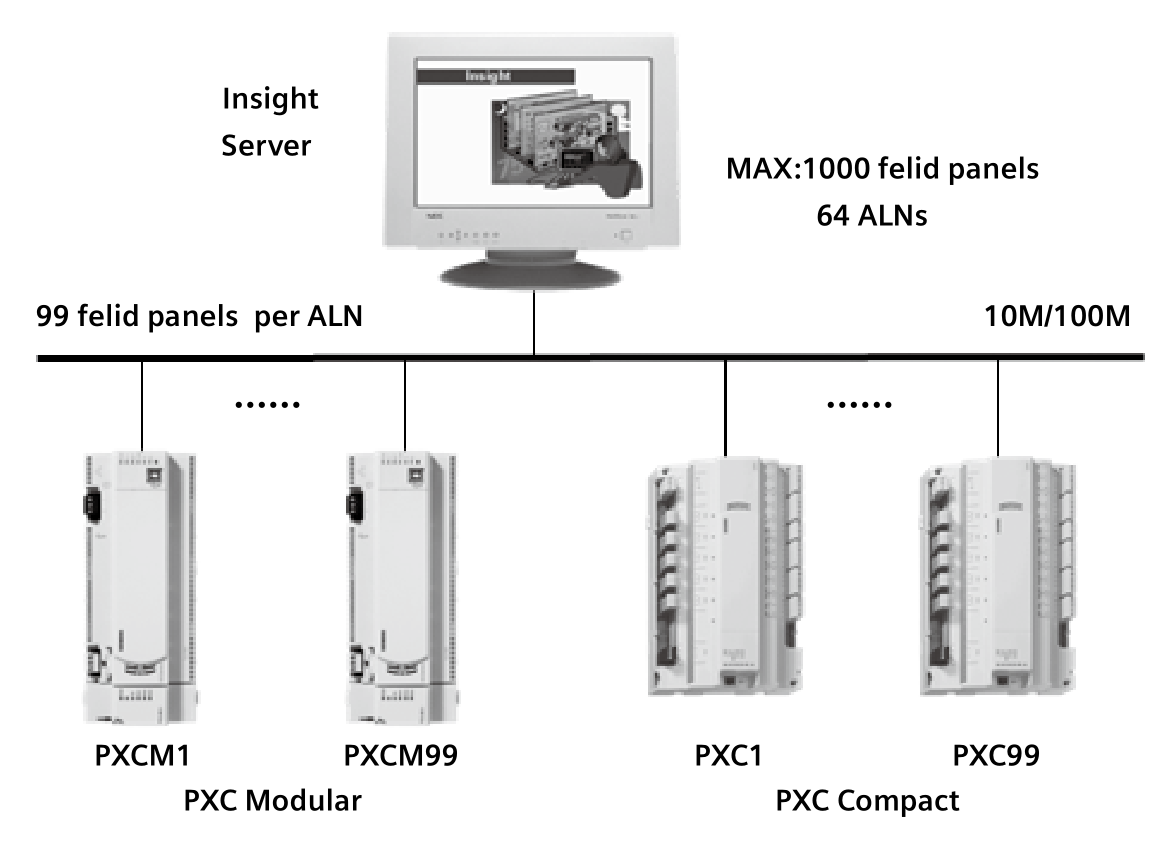
\includegraphics[scale=0.25]{img/framework.png}
      \end{center}
      \caption{基于以太网的两层构架APOGEE系统}\label{fig:fig1}
    \end{figure}

    一个典型的APOGEE系统由三层构架组成,包括管理级网络(Management Level Network),自控级网络(Automation Level Network)和现场级(Field LevelNetwork)网络。管理级网络指的是安装有监控软件的计算机组成的网络;自控级网络是由DDC控制器和Insight工作站组成的网络,ALN在组网上可以分为基于RS485组网方式和基于Ethernent组网方式,两种组网方式都支持西门子专有的P2通讯协议及标准的BACnet通讯协议;现场级网络主要是由终端设备控制器、点扩展模块等设备组成,也可以包括有通讯功能的现场设备组成的网络。其中自控层网络(ALN)是APOGEE系统的核心,由于高速的网络对DDC控制器处理复杂的控制任务有很大的好处,能在同一时间内采集和处理系统的各种控制信息,因此本次设计中采用基于Ethernet方式的ALN组网方式,与此同时为了保障五星级酒店设备控制的及时性和控制的可靠性,本次设计最终选择了基于以太网的两层构架APOGEE系统方案。其中,在MLN上,主要是Insight工作站,包括通常作为主控的Insight工作站服务器端,及通常作为分控的Insight工作站客户端。对于楼宇的能源使用情况有分析需求的项目,还需配置InfoCenter软件模块。工作在ALN层面上的控制器包括模块化PXC系列控制器PXCModular、16点紧凑型PXC系列控制器、24点紧凑型PXC系列控制器、36点紧凑型PXC系列控制器。关于DDC的具体规格,见\tabref{tab2}:

    \begin{table}[htbp]
      \zihao{5}
      \begin{center}
        \caption{DDC选型表}\label{tab:tab2}
        \begin{tabularx}{\linewidth}{c|Y|Y|Y|Y|Y|Y}
          \Xhline{1.5pt}
          \multirow{2}{*}{DDC型号} & \multicolumn{6}{c}{DDC点数分配} \\
          \cline{2-7}\multicolumn{1}{p{10em}|}{} & \multicolumn{1}{Y|}{UI} & \multicolumn{1}{Y|}{DI} & \multicolumn{1}{Y|}{AO} & \multicolumn{1}{Y|}{DO} & \multicolumn{1}{Y|}{U} & \multicolumn{1}{Y}{X} \\
          \hline
          PXC16.2-E.A & \multicolumn{1}{c|}{3} & 2 & 3 & 3 & 5 & 0 \\
          \hline
          PXC24.2-E.A & \multicolumn{1}{c|}{3} & 0 & 3 & 5 & 9 & 0 \\
          \hline
          PXC36-E.A & \multicolumn{1}{c|}{2} & 4 & 3 & 3 & 18 & 6 \\
          \hline
          TXM1.8D & \multicolumn{1}{c|}{0} & 8 & 0 & 0 & 0 & 0 \\
          \hline
          TXM1.8X & \multicolumn{1}{c|}{0} & 0 & 0 & 0 & 0 & 8 \\
          \hline
          TXM1.16D & \multicolumn{1}{c|}{0} & 16 & 0 & 0 & 0 & 0 \\
          \hline
          TXM1.6R & \multicolumn{1}{c|}{0} & 0 & 0 & 6 & 0 & 0 \\
          \hline
          PXX.485.3 & \multicolumn{6}{c}{RS-485扩展模块} \\
          \hline
          PXC100-E96.A & \multicolumn{6}{c}{PXC模块化可编程控制器} \\
          \hline
          TXS1.12F4 & \multicolumn{6}{c}{TX-I/O电源模块} \\
          \Xhline{1.5pt}
        \end{tabularx}
      \end{center}
    \end{table}

      \subsubsection{排烟风机}
      建筑内共有10台排烟风机,选用紧凑型PXC16.2-E.A进行控制,具体参数见\tabref{tab3}:

      \begin{table}[htpb]
        \begin{center}
          \caption{排烟风机监控点表}\label{tab:tab3}
          \begin{tabularx}{\linewidth}{c|c|Y|Y|Y|Y|Y|Y}
            \Xhline{1.5pt}
            数量 & 点数使用情况 & UI & DI & AO & DO & U & X \\
            \hline
            \multirow{2}{*}{10} & 提供I/O & 3 & 2 & 3 & 3 & 5 & 0 \\
            \cline{2-8}  & 实际I/O & 0 & 6 & 0 & 1 & 0 & 0 \\
            \Xhline{1.5pt}
          \end{tabularx}
        \end{center}
      \end{table}

      \subsubsection{排风机}
      建筑内共有12台排风机,选用紧凑型PXC16.2-E.A进行控制,具体参数见\tabref{tab4}:

      \begin{table}[htpb]
        \begin{center}
          \caption{排风机监控点表}\label{tab:tab4}
          \begin{tabularx}{\linewidth}{c|c|Y|Y|Y|Y|Y|Y}
            \Xhline{1.5pt}
            数量 & 点数使用情况 & UI & DI & AO & DO & U & X \\
            \hline
            \multirow{2}{*}{12} & 提供I/O & 3 & 2 & 3 & 3 & 5 & 0 \\
            \cline{2-8}  & 实际I/O & 0 & 4 & 0 & 1 & 0 & 0 \\
            \Xhline{1.5pt}
          \end{tabularx}
        \end{center}
      \end{table}

      \subsubsection{送风机}
      建筑内共有6台加压送风机与1台补风机,选用紧凑型PXC16.2-E.A进行控制,具体参数见\tabref{tab5}:

      \begin{table}[htpb]
        \begin{center}
          \caption{送风机监控点表}\label{tab:tab5}
          \begin{tabularx}{\linewidth}{c|c|Y|Y|Y|Y|Y|Y}
            \Xhline{1.5pt}
            数量 & 点数使用情况 & UI & DI & AO & DO & U & X \\
            \hline
            \multirow{2}{*}{7} & 提供I/O & 3 & 2 & 3 & 3 & 5 & 0 \\
            \cline{2-8}  & 实际I/O & 0 & 4 & 0 & 1 & 0 & 0 \\
            \Xhline{1.5pt}
          \end{tabularx}
        \end{center}
      \end{table}

      \subsubsection{全热交换机}
      建筑内共有6台全热交换机,选用紧凑型PXC36-E.A进行控制,具体参数见\tabref{tab6}:

      \begin{table}[htpb]
        \begin{center}
          \caption{全热交换机监控点表}\label{tab:tab6}
          \begin{tabularx}{\linewidth}{c|c|Y|Y|Y|Y|Y|Y}
            \Xhline{1.5pt}
            数量 & 点数使用情况 & UI & DI & AO & DO & U & X \\
            \hline
            \multirow{2}{*}{6} & 提供I/O & 0 & 4 & 0 & 8 & 18 & 6 \\
            \cline{2-8}  & 实际I/O & 10 & 5 & 2 & 2 & 0 & 0 \\
            \Xhline{1.5pt}
          \end{tabularx}
        \end{center}
      \end{table}

      \subsubsection{新风机组}
      建筑内共有3台新风机组,选用紧凑型PXC24.2-E.A进行控制,具体参数见\tabref{tab7}:

      \begin{table}[htpb]
        \begin{center}
          \caption{新风机组监控点表}\label{tab:tab7}
          \begin{tabularx}{\linewidth}{c|c|Y|Y|Y|Y|Y|Y}
            \Xhline{1.5pt}
            数量 & 点数使用情况 & UI & DI & AO & DO & U & X \\
            \hline
            \multirow{2}{*}{3} & 提供I/O & 3 & 0 & 3 & 5 & 9 & 4 \\
            \cline{2-8}  & 实际I/O & 4 & 6 & 3 & 2 & 0 & 0 \\
            \Xhline{1.5pt}
          \end{tabularx}
        \end{center}
      \end{table}

      \subsubsection{空调机组}
      建筑内共有8台空调机组,选用紧凑型PXC24.2-E.A进行控制,具体参数见\tabref{tab8}:

      \begin{table}[htpb]
        \begin{center}
          \caption{全热交换机监控点表}\label{tab:tab8}
          \begin{tabularx}{\linewidth}{c|c|Y|Y|Y|Y|Y|Y}
            \Xhline{1.5pt}
            数量 & 点数使用情况 & UI & DI & AO & DO & U & X \\
            \hline
            \multirow{2}{*}{8} & 提供I/O & 0 & 4 & 0 & 8 & 18 & 6 \\
            \cline{2-8}  & 实际I/O & 7 & 10 & 5 & 3 & 0 & 0 \\
            \Xhline{1.5pt}
          \end{tabularx}
        \end{center}
      \end{table}

      \subsubsection{消防给水系统}
      该酒店的消防给水设置在室外水泵房,包括了室外消防水池、喷淋泵、喷淋稳压泵、消防栓泵以及消防栓稳压泵等设备,每种水泵都是一用一备,用于增强系统的稳定性。由于设备数量比较多导致监控点数较大,因此选用模块化PXC100-E96.A与扩展模块进行控制。监控点具体参数见\tabref{tab9}:

      \begin{table}[htpb]
        \begin{center}
          \caption{消防给水系统监控点表}\label{tab:tab9}
          \begin{tabularx}{\linewidth}{c|c|Y|Y|Y|Y|Y|Y}
            \Xhline{1.5pt}
            位置 & 点数使用情况 & UI & DI & AO & DO & U & X \\
            \hline
            \multirow{2}{*}{室外水泵房} & 提供I/O & 0 & 24 & 0 & 6 & 8 & 0 \\
            \cline{2-8}  & 实际I/O & 0 & 24 & 0 & 8 & 0 & 0 \\
            \Xhline{1.5pt}
          \end{tabularx}
        \end{center}
      \end{table}

      此时消防水泵房选用的I/O模块包括:1个TXM1.16D,1个TXM1.8D,1个TXM1.6R,1个TXM1.8U,计算I/O模块所需总电流$\rm I=0.058+0.046+0.071+0.063=0.237A$,此时的电流大小小于$\rm 1.2A$,因此只需要提供一个TXS1.12F4电源模块。

      \subsubsection{排水系统}
      建筑内共有38台潜污泵,每台潜污泵和集水井中的水位检测器共同组成排水系统,选用紧凑型PXC16.2-E.A进行控制,具体参数见\tabref{tab10}。

      \begin{table}[htpb]
        \begin{center}
          \caption{排水系统监控点表}\label{tab:tab10}
          \begin{tabularx}{\linewidth}{c|c|Y|Y|Y|Y|Y|Y}
            \Xhline{1.5pt}
            数量 & 点数使用情况 & UI & DI & AO & DO & U & X \\
            \hline
            \multirow{2}{*}{38} & 提供I/O & 3 & 2 & 3 & 3 & 5 & 0 \\
            \cline{2-8}  & 实际I/O & 0 & 8 & 0 & 2 & 0 & 0 \\
            \Xhline{1.5pt}
          \end{tabularx}
        \end{center}
      \end{table}

      \subsubsection{冷源系统}
      该酒店的空调机房位于地下一层,包括了天面膨胀水箱、天面冷却塔、冷水机组、冷却水泵与冷水泵等设备,冷却水泵和冷水泵都是三用两备,用于增强空调系统的稳定性。此时也选用模块化PXC100-E96.A与扩展模块进行控制。监控点具体参数见\tabref{tab11}以及\tabref{tab12}:

      \begin{table}[htpb]
        \begin{center}
          \caption{冷源系统监控点表}\label{tab:tab11}
          \begin{tabularx}{\linewidth}{c|c|Y|Y|Y|Y|Y|Y}
            \Xhline{1.5pt}
            位置 & 点数使用情况 & UI & DI & AO & DO & U & X \\
            \hline
            \multirow{2}{*}{地下一层空调机房} & 提供I/O & 0 & 56 & 0 & 18 & 16 & 0 \\
            \cline{2-8}  & 实际I/O & 7 & 49 & 1 & 25 & 0 & 0 \\
            \Xhline{1.5pt}
          \end{tabularx}
        \end{center}
      \end{table}

      \begin{table}[htpb]
        \begin{center}
          \caption{冷源系统监控点表}\label{tab:tab12}
          \begin{tabularx}{\linewidth}{c|c|Y|Y|Y|Y|Y|Y}
            \Xhline{1.5pt}
            位置 & 点数使用情况 & UI & DI & AO & DO & U & X \\
            \hline
            \multirow{2}{*}{天面} & 提供I/O & 0 & 48 & 0 & 24 & 8 & 0 \\
            \cline{2-8}  & 实际I/O & 0 & 35 & 0 & 25 & 0 & 0 \\
            \Xhline{1.5pt}
          \end{tabularx}
        \end{center}
      \end{table}

      空调机房选用的I/O模块包括:3个TXM1.16D,1个TXM1.8D,3个TXM1.6R,2个TXM1.8U,计算I/O模块所需总电流$\rm I=0.058*3+0.046+0.071*3+0.063*2=0.559A$,此时的电流大小小于$\rm 1.2A$,只需要提供一个TXS1.12F4电源模块。

      空调机房选用的I/O模块包括:3个TXM1.16D,4个TXM1.6R,1个TXM1.8U,计算I/O模块所需总电流$\rm I=0.058*3+0.071*4+0.063=0.521A$,此时的电流大小小于$\rm 1.2A$,只需要提供一个TXS1.12F4电源模块。\clearpage

  \section{综合布线系统}
    \subsection{设计概况}
    综合布线系统下属有六个子系统,它们分别是工作区子系统、水平子系统、管理子系统、垂直干线子系统、设备室子系统以及建筑群子系统。至于本五星级酒店,由于只有单独一栋建筑,因此本次设计主要完成五个子系统的设计:工作区子系统、水平子系统、管理子系统、垂直干线子系统以及设备室子系统。

    设备室子系统是位于地下一层的电信机房,来自市政通信的进线光缆在电信机房分别通过数据核心交换机和语音网关处理,再由光纤配线架引出到弱电井,从弱电井引出到各层管理子系统。经过管理子系统的交换机以及配线架完成各种转换之后,经由水平子系统引至各信息点处而后转成工作区子系统。其中,工作区子系统共设有四种类型的信息点,它们分别是无线AP信息点、六类数据信息点、六类语音信息点以及光纤信息插座模块。每种信息点的数量以及位置根据相关规范以及工作区实际要求进行布置。建筑所需信息点统计如下\tabref{tab13}:

    \begin{table}[htpb]
      \begin{center}
        \caption{综合布线系统信息点统计}\label{tab:tab13}
        \begin{tabularx}{\linewidth}{>{\centering}p{4em}|c|c|c|c}
          \Xhline{1.5pt}
          楼层 & 无线AP信息点 & 六类数据信息点 & 六类语音信息点 & 光纤信息插座模块 \\
          \hline
          负一层 & 0 & 1 & 1 & 1 \\
          \hline
          首层 & 1 & 4 & 6 & 6 \\
          \hline
          二层 & 16 & 33 & 33 & 0 \\
          \hline
          三层 & 17 & 31 & 33 & 2 \\
          \hline
          四至十层 & 33 & 66 & 66 & 0 \\
          \hline
          十一层 & 29 & 56 & 56 & 0 \\
          \hline
          十二层 & 12 & 22 & 22 & 0 \\
          \hline
          天面层 & 1 & 1 & 1 & 0 \\
          \Xhline{1.5pt}
        \end{tabularx}
      \end{center}
    \end{table}

    管理子系统采用的交换机等设备的总数量如\tabref{tab14}所示:

    \begin{table}[htpb]
      \begin{center}
        \caption{综合布线系统设备统计}\label{tab:tab14}
        \begin{tabularx}{\linewidth}{Y|Y|c|c}
          \Xhline{1.5pt}
          设备名称 & \multicolumn{1}{p{4.19em}|}{设备数量} & 设备位置 & 备注 \\
          \hline
          数据核心交换机 & 1 & 地下一层电信机房 & 安装在弱电机柜内 \\
          \hline
          语音网关 & 1 & 地下一层电信机房 & 安装在弱电机柜内 \\
          \hline
          24口交换机 & 4 & 每层弱电井 & 安装在弱电机柜内 \\
          \hline
          48口交换机 & 36 & 每层弱电井 & 安装在弱电机柜内 \\
          \Xhline{1.5pt}
        \end{tabularx}
      \end{center}
    \end{table}

    \subsection{系统概述}
    本次综合布线系统完成的子系统设计仅包括五个部分,他们分别是:工作区子系统、水平子系统、管理子系统、垂直干线子系统以及设备室子系统。关于每个系统的设计概述如下:

    \begin{enumerate}[label={(\arabic*)}]
      \item 工作区子系统:工作区子系统是综合布线系统的末端,直接连接信息用户,其目的是实现工作区终端设备与水平子系统之间的连接,由终端设备连接到信息插座的连接线缆所组成。由信息插座、插座盒、连接跳线和适配器组成。工作区子系统的设计主要考虑信息插座和适配器两个方面。
      \item 水平子系统:水平子系统主要是指连接工作区子系统和管理子系统的中间子系统,水平子系统又被成为配线子系统,其目的是实现信息插座即工作区子系统和管理子系统间的连接,将用户工作区引至管理子系统,并为用户提供一个符合国际标准,满足语音及高速数据传输要求的信息点出口。
      \item 管理子系统:管理子系统是连接垂直干线子系统和水平子系统的重要中间子系统,针对建筑内的某一楼层而言,管理子系统相当于一个核心,该楼层内的所有末端综合布线均经过管理子系统与垂直干线子系统和设备室子系统相连接,因此,它的作用十分重要。管理子系统一般由由交连、互连配线架组成。管理点为连接其它子系统提供连接手段。交连和互连允许将通讯线路定位或重定位到建筑物的不同部分,以便能更容易地管理通信线路,使在移动终端设备时能方便地进行插拔。互连配线架根据不同的连接硬件分楼层配线架(箱)IDF和总配线架(箱)MDF,IDF可安装在各楼层的干线接线间,MDF一般安装在设备机房。
      \item 垂直干线子系统:垂直干线子系统是连接管理子系统与设备室子系统的重要干线子系统,其目的是实现计算机设备、程控交换机、控制中心与各管理子系统间的连接,是建筑物干线电缆的路由。该子系统通常是两个单元之间,特别是在位于中央点的公共系统设备处提供多个线路设施。系统由建筑物内所有的垂直干线多对数电缆及相关支撑硬件组成,以提供设备间总配线架与干线接线间楼层配线架之间的干线路由。常用介质是大对数双绞线电缆和光缆。
      \item 设备室子系统:设备室子系统是连接垂直干线子系统和建筑群子系统的核心下属子系统,其位置非常重要。该子系统能够统一管理建筑的线缆,进行语音、数据、光纤信息点的总分配。一般而言,设备室子系统主要由电缆、连接器和有关的支撑硬件组成,作用是将计算机、PBX、摄像头、监视器等弱电设备互连起来并连接到主配线架上。设备包括计算机系统、网络集线器、网络交换机、程控交换机、音响输出设备、闭路电视控制装置和报警控制中心等。
    \end{enumerate}

    \subsection{设计原则}
    通过查阅相关规范,综合布线系统的设计应遵循以下原则:
    \begin{enumerate}[label={(\arabic*)}]
      \item 综合布线系统工程的产品类别及链路、信道等级的确定应综合考虑建筑物的性质、功能、应用网络和业务对传输带宽及缆线长度的要求、业务终端的类型、业务的需求及发展、性能价格、现场安装条件等因素,并应符合规范\cite{s2}中的规定。
      \item 同一布线信道及链路的缆线、跳线和连接器件应保持系统等级与阻抗的一致性。
      \item 综合布线系统光纤信道应采用标称波长为850nm和1300nm的多模光纤(OM1、OM2、OM3、OM4),标称波长为1310nm和1550nm(OS1),1310nm、1383nm和1550nm(OS2)的单模光纤。单模和多模光缆的选用应符合网络的构成方式、业务的互联方式、以太网交换机端口类型及网络规定的光纤应用传输距离。在楼内宜采用多模光缆,超过多模光纤支持的应用长度或需直接与电信业务经营者通信设施相连时应采用单模光缆。
      \item 配线设备之间互连的跳线宜选用产业化制造的产品,跳线的类别应符合综合布线系统的等级要求。在应用电话业务时宜选用双芯对绞电缆。
      \item 工作区信息点为电端口时应采用8位模块通用插座,光端口应采用SC或LC光纤连接器件及适配器。
      \item CP集合点安装的连接器件应选用卡接式配线模块或8位模块通用插座或各类光纤连接器件和适配器。
      \item 综合布线系统产品的选用应考虑缆线与器件的类型、规格、尺寸对安装设计与施工造成的影响。
    \end{enumerate}

    \subsection{设备选型}
    作为五星级酒店,本建筑的综合布线系统设计优先考虑的是支持用户通信网络的使用要求,能让用户正常方便地使用万兆局域网;另一方面,要保证设备运行的稳定性,不会因为突发情况造成严重后果;除此之外,选用设备一定要具有完善的防火墙功能,以便保障酒店本身以及顾客的相关数据;最后所选设备的能耗要尽量低。选择的设备如下\tabref{tab15}所示

    \begin{table}[htpb]
      \begin{center}
        \caption{综合布线系统设备选型}\label{tab:tab15}
        \begin{tabularx}{\linewidth}{c|c|Y}
          \Xhline{1.5pt}
          设备名称 & 设备型号 & 设备参数 \\
          \hline
          数据核心交换机 & H3C S6890-54HF & 48个SFP Plus口,6个QSFP28口,两个带外管理以太网口(一光一电) \\
          \hline
          语音网关 & H3C ICG 5000 & 3个固定GE口,4个SIC插槽,2个DSIC,4个HMIM插槽以及2个VPM \\
          \hline
          24口交换机 & H3C S5560-30S-EI & 24个10/100/1000Base-T自适应以太网端口,4个万兆SFP+口以及2个40G QSFP+口 \\
          \hline
          48口交换机 & H3C S5560-54S-EI & 48个10/100/1000Base-T自适应以太网端口,4个万兆SFP+口以及2个40G QSFP+口 \\
          \Xhline{1.5pt}
        \end{tabularx}
      \end{center}
    \end{table}

    \subsection{设计方案}
      \subsubsection{工作区子系统}
      工作区的设计主要是确定无线信息点、数据信息点以及语音信息点,同时根据房间的功能决定是否需要预留光纤信息插座模块。对于客房和包间,考虑到顾客仅仅需要在床边和书桌附近使用数据和语音,因此直接在房间中这两个位置附近布置数据信息点和语音信息点即可,同时每个房间布置一个无线AP信息点以便提供无线上网功能。对于办公室和会议室,考虑到沿墙敷设的局限,每个房间沿墙边各提供一个语音和一个数据信息点的同时,根据房间的功能决定是否预留一个光纤信息插座模块以提供可扩展的能力。为了保持系统的灵活性和稳定性,数据信息点和语音信息点都采用六类UTP连接。

      \subsubsection{水平子系统}
      水平子系统即配线子系统采用的是最常见的拓扑星型结构以确保信息用户的独立性和信息交换的可靠性。工作区子系统出来后,通过网线、电话线、光纤布线形成水平子系统,走线方式有埋地、沿墙、吊顶、跨柱等,而后再与管理子系统中的配线架相互连接,形成工作区子系统到水平子系统再到管理子系统的一体连接。线型均采用通用标准型光纤、光缆、六类UTP网线。

      \subsubsection{管理子系统}
      管理子系统主要包括了配线架和网络交换机两个部分。其中,配线架包括:光纤配线架和六类配线架,配线架的作用主要是实现线缆分配与管理,具体配线架的型号可参看系统图,均采用通用标准型口数配线架;交换机的作用是实现光电转化与数据交换,同时作为网络架构第二层的设备实现网关、VLAN等功能。

      \subsubsection{垂直干线子系统}
      由于数据信息点和语音信息点都采用了六类UTP的传输形式,因此本系统使用室内多模光纤作为垂直干线子系统,线缆在弱电井内贴墙敷设,并配备相应的保护措施。

      \subsubsection{设备室子系统}
      分别选取一个数据用核心交换机和一个语音网关作为数据和语音的总接入处理,除此之外设备室子系统中还需要配备相应的服务器与管理工作站以及防火墙设备,用来实现对接入网络的控制和管理。\clearpage

  \section{安防系统}
    \subsection{设计概况}
    安防系统下属有三个小的系统,它们分别是视频监控系统、防盗报警系统以及门禁控制系统,由于本次设计选择了带有防区报警模块的门禁控制主机,因此门禁系统主机同时作为报警主机使用,如此一来本次设计仅需要完成两个主要的系统设计。

    安防系统监控中心设置在首层消防控制室并由控制室引出门禁控制线和监控控制线到弱电井,而后再经弱电井在垂直方向上敷设至各层并引至各末端设备。

    门禁报警系统采用的门禁主机又分为单门式、双门式和四门式,以及与之连接的各个模块设备。各个设备与总数量见下\tabref{tab16}:

    \begin{table}[htpb]
      \begin{center}
        \caption{门禁报警系统设备统计}\label{tab:tab16}
        \begin{tabularx}{\linewidth}{c|c|c|Y}
          \Xhline{1.5pt}
          设备名称 & \multicolumn{1}{p{4.69em}|}{设备数量} & 设备位置 & 备注 \\
          \hline
          单门禁控制主机 & 293 & 室内墙壁 & 嵌入墙内 \\
          \hline
          双门禁控制主机 & 38 & 室内墙壁 & 嵌入墙内 \\
          \hline
          四门禁控制主机 & 20 & 室内墙壁 & 嵌入墙内 \\
          \hline
          开门按钮 & 371 & 室内墙壁 & 嵌入墙内 \\
          \hline
          读卡器 & 371 & 室外墙壁 & 嵌入墙内 \\
          \hline
          门磁 & 429 & 房间门 & 安装在门和门框上 \\
          \hline
          电控锁 & 429 & 房间门 & 安装在门上 \\
          \hline
          双鉴探测器 & 371 & 室内墙壁 & 壁挂 \\
          \hline
          梯控主机 & 1 & 电梯机房 & 安装在机柜内 \\
          \hline
          梯控联动模块 & 2 & 电梯机房 & 安装在机柜内 \\
          \hline
          8口交换机 & 1 & 弱电井 & 安装在机柜内 \\
          \hline
          16口交换机 & 1 & 弱电井 & 安装在机柜内 \\
          \hline
          24口交换机 & 2 & 弱电井 & 安装在机柜内 \\
          \hline
          48口交换机 & 10 & 弱电井 & 安装在机柜内 \\
          \Xhline{1.5pt}
        \end{tabularx}
      \end{center}
    \end{table}

    视频监控系统选用了三种监摄像头:球机、半球及以及枪式机。每种摄像头都支持POE供电,因此还需要选择具有POE功能的交换机。设备具体参数与数量见下\tabref{tab17}:

    \begin{table}[htpb]
      \begin{center}
        \caption{视频监控系统设备统计}\label{tab:tab17}
        \begin{tabularx}{\linewidth}{c|c|c|Y}
          \Xhline{1.5pt}
          设备名称 & \multicolumn{1}{p{4.69em}|}{设备数量} & 设备位置 & 备注 \\
          \hline
          全球摄像机 & 1 & 二层 & 吸顶安装 \\
          \hline
          半球摄像机 & 93 & 地上各楼层 & 吸顶安装 \\
          \hline
          枪式摄像机 & 13 & 地下一层 & 支架壁装 \\
          \hline
          8口POE交换机 & 8 & 弱电井 & 安装在机柜内 \\
          \hline
          16口POE交换机 & 4 & 弱电井 & 安装在机柜内 \\
          \hline
          24口POE交换机 & 1 & 弱电井 & 安装在机柜内 \\
          \hline
          NVR & 1 & 消防控制室 & 安装在机柜内 \\
          \hline
          LCD液晶显示单元 & 16 & 消防控制室 & 安装在电视墙上 \\
          \hline
          控制键盘 & 1 & 消防控制室 & 安装在机柜内 \\
          \Xhline{1.5pt}
        \end{tabularx}
      \end{center}
    \end{table}

    \subsection{系统概述}
    考虑到系统的完整性,门禁报警系统、视频监控系统能够通过厂家提供的软件服务实现联动,进一步增强系统的可靠性,全套设备与软件都选择国内知名品牌海康威视。

    在软件方面,使用iVMS-4200 AC客户端,它是为门禁、考勤和可视对讲业务开发的的软件应用程序。可与门禁控制器、门口机、室内机、报警主机等配套使用,支持设备管理、人员管理、远程配置、事件接收和联动、访问控制、考勤管理、日志查询等多种功能。提供灵活、多样的部署方案;与此同时配套使用iVMS-4200,它是一款与嵌入式网络监控设备配套使用的应用软件。它可与DVR、NVR、IPC、IPD、DVS、网络存储设备、报警设备、门禁设备、可视对讲设备等配套使用,提供灵活、多样的部署方案,满足中、小型项目中各种不同环境的需求。除此之外,厂家提供移动端软件服务,即iVMS-4500视频监控客户端,它可通过无线网络,实现对硬盘录像机、视频服务器、热成像设备、网络摄像机和网络球机的实时图像预览、远程录像回放、云台控制、本地图片和录像存储、报警推送信息管理等功能。同时客户端软件支持萤石云,在客户端上登录萤石云账号后,可对与此账号关联的萤石设备进行管理。iVMS-4500软件支持Wi-Fi,3G或4G网络等连接方式。

    门禁系统作为安防系统里最重要的一环,直接决定了酒店的安全水平。传统的门禁系统功能较为单一,稳定性和可扩展性不高,而随着科技水平的不断发展,人们对系统的先进性、易用性要求越来越高,各种新式门禁设备层出不穷,伴随着这些设备发展而来的,便是综合安防解决方案。综合安放解决方案的特点,便是用相同的设备,配合完整的系统以及软件,完成更多的功能,实现安防系统的“高内聚”。为了顺应这股“大安防”的潮流,在本次设计中综合考虑了门禁系统和报警系统单独布置,门禁报警一体化等多个方案,最终确定以门禁报警一体化作为本酒店的实施方案。由于酒店客房较多,单独布置的防盗报警系统成本高、难维护,不方便管理,因此采用门禁报警一体化系统的方式,既降低了系统施工的成本,又加强了两个系统之间的联系,同时更利于管理和维护。本酒店门禁系统采用单向感应式系统,使用者在门外出示经过授权的感应卡,经读卡器识别确认合法身份后,控制器驱动打开电锁放行,并记录进门时间。按开门按钮,打开电锁,直接外出。根据酒店房间的不同类型,分别采用单门、双门、四门控制主机,门禁控制主机置于室内,暗装于门旁边的墙体内。安装于门旁附近墙体标高2米左右的双鉴探测器接入门禁控制主机的4防区防盗报警输入,实现了防盗报警系统和门禁控制系统的统一。为了方便未来对门禁系统的升级改造以及实现弱电系统的综合控制,本门禁系统采用基于TCP/IP协议的星型连接方式,由布置在消防控制室的总交换机拉线至各层弱电井中的交换机,进而连接到各个门禁控制主机。与BA系统的DDC一样,门禁控制主机通过UPS进行独立供电。

    视频监控系统对于本次安防系统设计同样非常重要,为能够保证视频数据传输量,本次设计采用网络摄像头作为监控末端并根据不同的使用环境确定了三种摄像末端,它们分别是球式摄像机,半球摄像机以及枪式摄像头。其中,球式摄像机主要应用于人员密集需要迅速捕捉影像的地点,本次设计中即酒店首层大堂;半球摄像机主要应用于走廊、楼梯、电梯间等地点的监控;枪式摄像机则应用于地下车库。由于本视频监控系统采用POE的方式供电,因此三种监控摄像机都选用支持POE供电模式的摄像机。消防控制室通过设置NVR\&解码上墙一体机代替传统NVR+视频矩阵的方式,既可作为NVR进行本地独立工作,也可进行电视墙的拼控管理,同时可联网组成一个强大的安全防范系统。

    \subsection{设计原则}
    通过查阅相关规范,安防系统的设计应遵循以下原则:
    \begin{enumerate}[label={(\arabic*)}]
      \item 楼宇安防系统的设计应以实用为第一原则。在能够达到安全要求的前提下,合理平衡系统的经济性与超前性,以避免片面追求超前性而脱离实际,或片面追求经济性而损害综合楼的安全性。
      \item 系统必须保持每天24小时连续工作。子系统故障不影响其他子系统运行,也不影响集成系统除该子系统之外的其他功能的运行。
      \item 本楼宇安防系统方案所选用的设备与系统,是以现有成熟的设备和系统为基础的设备与系统。在楼宇安防系统工程投资中,以总体目标为方向,局部服从全局,力求系统在初次投入和整个运行生命周期获得最佳的性能/价格比。
      \item 因为本系统极为复杂,要保证日常运行,系统必须具有高度的可维护性和易维护性,尽量做到所需维护人员少,维护工作量小,维护强度低,维护费用低。
      \item 本楼宇安防系统设计尽量采用国家和国际标准及规范,兼容不同厂商、不同协议的设备和系统的信号传输,各子系统可方便进出系统。
    \end{enumerate}

    \subsection{设备选型}
    本次安防设计的基本设备全部采用海康威视,交换机等网络交换设备采用新华三(H3C)。

      \subsubsection{门禁报警系统}
      门禁系统选用了海康威视DS-K2600系列门禁控制主机,该控制主机具有如下特征:

      \begin{enumerate}[label={(\arabic*)}]
        \item 32位高速处理器,TCP/IP和RS485通讯方式,支持HIK ehome协议实现数据跨公网通讯。
        \item 可存储10万笔合法卡,30万笔刷卡记录。
        \item 支持多门互锁、反潜回、多重卡开门、首卡开门、超级卡和超级密码开门、密码开门、在线升级、中心远程开门等功能。
        \item 具有读卡器防拆、门未关妥报警、门被外力开起、开门等待超时、胁迫卡和胁迫码、黑名单、非法卡超次刷卡报警等多种报警机制。
        \item 支持RS485接口和韦根接口读卡器的接入。
        \item 支持普通卡/残疾人卡/黑名单/巡更卡/来宾卡/胁迫卡/超级卡等多种卡片类型。
        \item 支持4防区报警输入,具有防短、防剪功能。
        \item 内建RTC,支持NTP校时、手动校时、自动校时功能。
        \item 支持脱机记录保持功能和纪录储存空间不足警告功能。
        \item 主机具有备用电池设计,外部供电断开时可不间断切换蓄电池供电,保障门禁系统正常运行。
      \end{enumerate}

      通过该主机组成的门禁控制系统如下\figref{fig2}所示:
      \begin{figure}[htpb]
        \begin{center}
          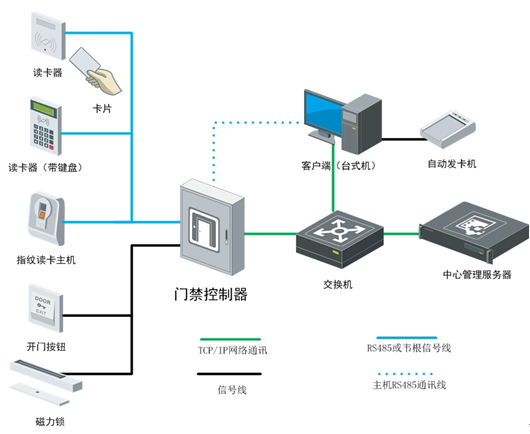
\includegraphics[scale=0.8]{img/access_control.png}
        \end{center}
        \caption{DS-K2600系列门禁主机的典型应用}\label{fig:fig2}
      \end{figure}

      作为门禁系统的子系统,本次设计中的梯控系统采用了海康威视DS-K2210梯控主机以及DS-K2M0016A梯控联动模块,该梯控主机与模块具有如下特点:

      \begin{enumerate}[label={(\arabic*)}]
        \item 可实现128层进出权限的管控。
        \item 支持接入2个Wiegand读卡器或RS485读卡器。
        \item 支持2W笔合法卡以及5W笔存储记录的存储。
        \item 支持Web管理,实现权限操作、楼层配置、参数配置、远程操作。
        \item 支持通过事件(消防、紧急、维护)输入,配置完成事件联动输出。
        \item 支持防拆报警功能。(仅带机箱支持)。
        \item 支持NTP校时、手动校时、自动校时功能。
        \item 支持事件上传,脱机工作后支持离线事件存储,断电后数据可以永久保存。
        \item 具有看门狗检测功能,保障主机长期稳定运行。
        \item 模块通过RS-485与梯控主板实现通信,具有16路继电器输出,一个模块最多可控制16层电梯。
        \item 模块通过拨码开关设置梯控联动模块类型(呼梯/按键/自动)。
        \item 模块通过继电器的开关达到楼层控制的目的,且继电器变化的状态可上传梯控主板。
      \end{enumerate}

      关于门禁系统中各个子设备,详见设备选型表\tabref{tab18}:

      \begin{table}[htpb]
        \begin{center}
          \caption{门禁报警系统设备选型}\label{tab:tab18}
          \begin{tabularx}{\linewidth}{c|c|Y}
            \Xhline{1.5pt}
            设备名称 & 设备型号 & 备注 \\
            \hline
            单门禁控制主机 & DS-K2601 & DC12V \\
            \hline
            双门禁控制主机 & DS-K2602 & DC12V \\
            \hline
            四门禁控制主机 & DS-K2604 & DC12V \\
            \hline
            读卡器 & DS-K1101 & DC12V,功耗≤2W \\
            \hline
            门磁 & DS-1T610N & 动作距离≥35mm \\
            \hline
            电控锁 & DS-K4T600C & DC12V \\
            \hline
            双鉴探测器 & KX10DTP & DC9-16V,红外+微波 \\
            \hline
            梯控主机 & DS-K2210 & DC12V \\
            \hline
            梯控联动模块 & DS-K2M0016A & DC12V \\
            \hline
            8口安防交换机  & H3C MS4010 & 100-240V AC,最大功耗0.006kW \\
            \hline
            16口安防交换机 & H3C MS4016 & 100-240V AC,最大功耗0.02kW \\
            \hline
            24口安防交换机 & H3C MS4024P & 100-240V AC,最大功耗0.02kW \\
            \hline
            48口安防交换机 & H3C MS4048P & 100-240V AC,最大功耗0.02kW \\
            \Xhline{1.5pt}
          \end{tabularx}
        \end{center}
      \end{table}

      \subsubsection{视频监控系统}
      作为视频监控系统最核心的NVR,选用了海康威视的DS-96000系列NVR\&解码上墙一体机,该主机具有以下特点:

      \begin{enumerate}[label={(\arabic*)}]
        \item 集成存储、解码显示、拼接控制、智能分析等多种功能于一体,一机多用,部署简单,功能齐全。
        \item 专业的嵌入式软硬件设计,系统运行稳定可靠。
        \item 冗余电源、全插拔模块化设计,充分保障系统运行、维护的便捷可靠。
        \item 支持硬盘热插拔,支持RAID0、RAID1、RAID5,RAID6,RAID10,支持全局热备盘。
        \item 支持网络摄像机断网智能补录(ANR)和热备功能,提升数字通道存储的可靠性。
        \item 支持1200W像素高清网络视频的预览、存储与回放。
        \item 支持768Mbps输入带宽,最大可接入128路/256路高清网络视频。
        \item 支持接驳符合ONVIF、RTSP协议及众多主流厂商的网络摄像机。
        \item 支持多个HDMI、VGA口同时输出,且可分别预览或回放不同通道的图像。
        \item 支持24个SATA接口,1个eSATA接口,可选配miniSAS高速扩展接口,充分满足高清存储所需硬盘空\item 间。
        \item 可选配接口扩展板,支持4个千兆光口,8个RS-485串行接口,32进16出报警接口。
        \item 支持海康SMART IPC越界、进入区域、离开区域、区域入侵、徘徊、人员聚焦、快速移动、非法停车、物品遗留、物品拿取、音频输入异常、声强突变、虚焦以及场景变更等多种智能侦测接入与联动;支持智能搜索、回放及备份功能,有效提高录像检索与回放效率。
        \item 支持USB 3.0接口,充分满足高速备份需求。
      \end{enumerate}

      通过该主机组成的视频监控系统如下\figref{fig3}所示。
      \begin{figure}[htpb]
        \begin{center}
          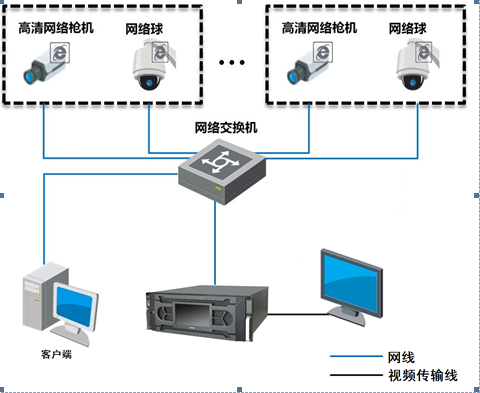
\includegraphics[scale=0.5]{img/monitoring.png}
        \end{center}
        \caption{DS-96000系列解码上墙一体机的典型应用}\label{fig:fig3}
      \end{figure}

      全球摄像机选用海康威视300万像素红外网络高清高速智能球机,其具体特点有:支持最大2048×1536@30fps高清画面输出,支持H.265高效压缩算法,可较大节省存储空间,支持超低照度,0.02Lux/F1.6(彩色),0.002Lux/F1.6(黑白) ,0 Lux with IR,支持30倍光学变倍,16倍数字变倍,采用高效红外阵列,低功耗,照射距离达180m,支持1080p@60fps、960p@60fps、720p@60fps高帧率输出,支持三码流技术,每路码流可独立配置分辨率及帧率,支持区域入侵侦测、越界侦测、移动侦测等智能侦测功能,支持手动跟踪、全景跟踪、事件跟踪,并支持多场景巡航跟踪,支持车牌捕获及检索、多场景巡航检测、云存储服务功能,支持断网续传功能保证录像不丢失,配合Smart NVR实现事件录像的二次智能检索、分析和浓缩播放,支持3D数字降噪、宽动态、透雾、强光抑制、SmartIR等功能,支持360°水平旋转,垂直方向-2°-90°,支持300个预置位,8条巡航扫描,支持3D定位,可通过鼠标框选目标以实现目标的快速定位与捕捉,支持定时抓图与事件抓图功能,支持定时任务、一键守望、一键巡航功能,支持雨刷功能,内置光模块,支持FC光纤接口与以太网电口输出,支持Hi-PoE供电,支持1路音频输入和1路音频输出,内置7路报警输入和2路报警输出,支持报警联动功能,支持最大128G的Micro SD/SDHC/SDXC卡存储,支持海康SDK、ONVIF、CGI、PSIA、GB/T28181和E家协议接入,防雷、防浪涌、防突波,IP66防护等级。

      半球摄像机采用海康威视日夜型半球网络摄像机,其具体特点有:最高分辨率可达5M(2560×1920 @ 12.5 fps),并可输出3M(2048×1536 @ 25 fps)实时图像,支持低码率、低延时、ROI感兴趣区域增强编码、SVC自适应编码技术,支持smart265编码,码流平滑设置,适应不同场景下对图像质量、流畅性的不同要求,支持GBK字库,支持更多汉字及生僻字叠加,支持OSD颜色自选,高效红外灯,使用寿命长,照射距离可达10-30米,支持smart IR,防止夜间红外过曝,ICR红外滤片式自动切换,实现真正的日夜监控,支持日夜两套参数独立配置,支持POE供电功能,支持Micro SD/SDHC/SDXC卡(128G)本地存储,支持Wi-Fi功能,支持3D数字降噪, 支持数字宽动态,支持三码流,支持手机监控,支持背光补偿,自动电子快门功能,适应不同监控环境,功能齐全:心跳,镜像,一键恢复等,支持多种智能报警,内置一对麦克风、喇叭,支持语音对讲,支持1对报警输入/输出(-S),支持智能后检索,配合NVR支持事件的二次检索分析,支持GB28181接入,支持E家平台接入,支持萤石云平台接入,支持NAS、Email、FTP、NTP服务器测试,支持HTTPS等安全认证,支持创建证书,初始设备开机修改密码,保障密码安全,支持用户登录锁定机制,及密码复杂度提示,防暴:防暴等级支持IK10。

      枪型摄像机选用海康威视日夜枪型网络摄像机,其特点有:最高分辨率可达1920×1080 @ 30 fps,在该分辨率下可输出实时图像,采用ROI等视频压缩技术,压缩比高,且处理非常灵活,超低码率,码流平滑设置,适应不同场景下对图像质量、流畅性的不同要求,支持GBK字库,支持更多汉字及生僻字叠加,支持OSD颜色自选,支持Micro SD/SDHC/SDXC卡(128G)本地存储,ICR红外滤片式自动切换,实现真正的日夜监控,支持日夜两套参数独立配置,支持POE供电功能,支持3D数字降噪,支持120dB超宽动态,支持双码流,支持手机监控,支持走廊模式,背光补偿,自动电子快门功能,适应不同监控环境,功能齐全:心跳,镜像,一键恢复等,支持智能报警:越界侦测,区域入侵侦测,支持智能后检索,配合NVR支持事件的二次检索分析,支持GB28181接入,支持EHOME平台接入,支持EZVIZ平台接入,支持NAS、Email、FTP、NTP服务器测试,支持HTTPS,SSH等安全认证,支持创建证书,支持用户登录锁定机制,及密码复杂度提示。

      系统中的其他设备,详见设备选型表\tabref{tab19}

      \begin{table}[htpb]
        \begin{center}
          \caption{视频监控系统设备选型}\label{tab:tab19}
          \begin{tabularx}{\linewidth}{c|c|Y}
            \Xhline{1.5pt}
            设备名称 & 设备型号 & 备注 \\
            \hline
            全球摄像机 & DS-2DF7330IW & 300万像素红外网络高清高速 \\
            \hline
            半球摄像机 & DS-2CD2336F(D)WD-IS & 300万星光级1/2.8”CMOS ICR日夜型 \\
            \hline
            枪式摄像机 & DS-2CD2T36F(D)WD-I8S & 300万星光级1/2.8”CMOS ICR红外阵列 \\
            \hline
            8口POE交换机 & H3C MS4010-HPWR & 100-240V AC,最大功耗0.15kW \\
            \hline
            16口POE交换机 & H3C MS4016-PWR & 100-240V AC,最大功耗0.21kW \\
            \hline
            24口POE交换机 & H3C MS4024P-PWR & 100-240V AC,最大功耗0.23kW \\
            \hline
            NVR & DS-96128 &  AC100V~240V,功耗≦140W \\
            \hline
            LCD 液晶显示单元 & DS-D2046NL-B/Z &   AC100V~240V,功耗≦130W \\
            \hline
            控制键盘 & DS-1200K & DC12V,功耗≦4.5W \\
            \Xhline{1.5pt}
          \end{tabularx}
        \end{center}
      \end{table} \clearpage

  \section*{总 \quad 结}
  \addcontentsline{toc}{section}{总结}
  经过一个多月的紧张设计,从一开始的茫然不解,到现在的如指诸掌,我从这次弱电毕设中学到非常多的知识。

  首先是关于对系统图的认识,最开始我认为系统图就是一个系统方案的示意图,大概表述清楚即可,具体的内容在平面图上表示。经过这段时间的学习,我终于意识到,系统图才是一个系统设计的核心,一个好的系统图才能成就一个好的方案。

  其次是学习到了一个完整弱电系统的设计过程。在开始设计之前,我一直认为弱电设计和强电设计类似,大抵都是“计算、校核、线路敷设”这样的过程。而实际上,这两者相差得还是比较远的,强电讲究的是计算,更偏向于理论,而弱电注重的是系统的设计,更偏向于应用。目前为止,我已经成功掌握了BA系统、综合布线系统、安防系统这弱电三大系统的设计方法和步骤,至于其他的系统,大都和这三大系统的设计过程类似,因此掌握了这三个大系统的设计过程,之后遇上弱电设计就不需要担心如何下手的问题了。

  最后,此次毕业设计锻炼了对知识的综合运用能力,以及自己收集资料并学习消化的能力,我觉得这才是毕业设计带给我最大的收获。\clearpage

  \begin{thebibliography}{}
    \bibitem[1]{s1} GB50348—2018, 安全防范工程技术规范[S]. 北京:中国计划出版社,2018.
    \bibitem[2]{s2} GB 50311-2016, 综合布线系统工程设计规范[S]. 北京:中国建筑工业出版社,2016.
    \bibitem[3]{s3} JGJ16­2008, 民用建筑电气设计规范[S]. 北京:中国建筑工业出版社,2008.
    \bibitem[4]{s4} GB50396-2007, 出入口控制系统工程设计规范[S]. 北京:中国计划出版社,2007.
    \bibitem[5]{s5} GB50395-2007, 视频安防监控系统工程设计规范[S]. 北京:中国计划出版社,2007.
    \bibitem[6]{s6} GB50394-2007, 入侵报警系统工程设计规范[S]. 北京:中国计划出版社,2007.
    \bibitem[7]{s7} GB50016-2014, 建筑设计防火规范[S]. 北京:中国计划出版社,2014.
    \bibitem[8]{s8} GB50314-2015, 智能建筑设计标准[S]. 北京:中国计划出版社,2015.
    \bibitem[9]{b1} 09X700(上), 智能建筑弱电工程设计与施工 (上册 )[M]. 北京:中国建筑标准设计研究院,2009.
    \bibitem[10]{b2} 09X700(下), 智能建筑弱电工程设计与施工 (下册 )[M]. 北京:中国建筑标准设计研究院,2009.
    \bibitem[11]{b3} 中国建筑标准设计研究所, 全国民用建筑工程技术措施-电气[M]. 北京:中国计划出版社,2009.
    \bibitem[12]{a1} Zhiwen Pan and Salim Hariri and Jesus Pacheco. Context aware intrusion detection for building automation systems[J]. Computers \& Security,2019,85:181-201.
    \bibitem[13]{a2} P. Zhang, X. Liu and L. Tao, Design of Security Access Control System of Adaptive Wireless Gateway[J]. International Symposium on Information Science and Engineering,2008,2:20-23.
  \end{thebibliography}\clearpage

  \section*{致 \quad 谢}
  \addcontentsline{toc}{section}{致谢}
  四年的大学学习生活在即将划上一个句号,而于我的人生来说却仅仅只是一个逗号,我将面对新的征程的开始。

  这次毕业设计是在屠宇老师的耐心的指导下完成的,也许我不是您最出色的学生,但您却是我所最喜爱的老师。屠老师平易近人,对学生充满耐心,事无巨细地回答了我毕业设计中遇到的各种问题,虽然屠老师的严格要求让我疲惫不已,但同时这让我的设计更加的严谨。于此同时,我还要感谢校外的谢远溪老师为我们提供的设计资料与校外辅导,这对我能顺利完成此次毕业设计起到了非常关键的作用。

  同时,我还要感谢一下一起完成毕业论文小组的同学们,如果没有你们的支持和倾心的协助,我是无法解决这些困难和疑惑,最终能够让本文顺利完成。至此论文付梓之际,我的心情无法保持平静,从开始选择课题到论文的顺利答辩,有无数可敬的师长、朋友给了我很多的帮助,在这里请您接受我诚挚的谢意!

  最后,再次对那些在论文完成过程中,关心、帮助我的同学和朋友们表示衷心地感谢!
\end{document}
